%introduction used to set the whole 

\documentclass{article}
\title{hw1}
\author{Wenhua Bao 2512664\\Yue Liu 2803140}
\usepackage{graphicx}
\usepackage{pdfpages}

%TEXT
\begin{document}
\maketitle
\section{Task1}
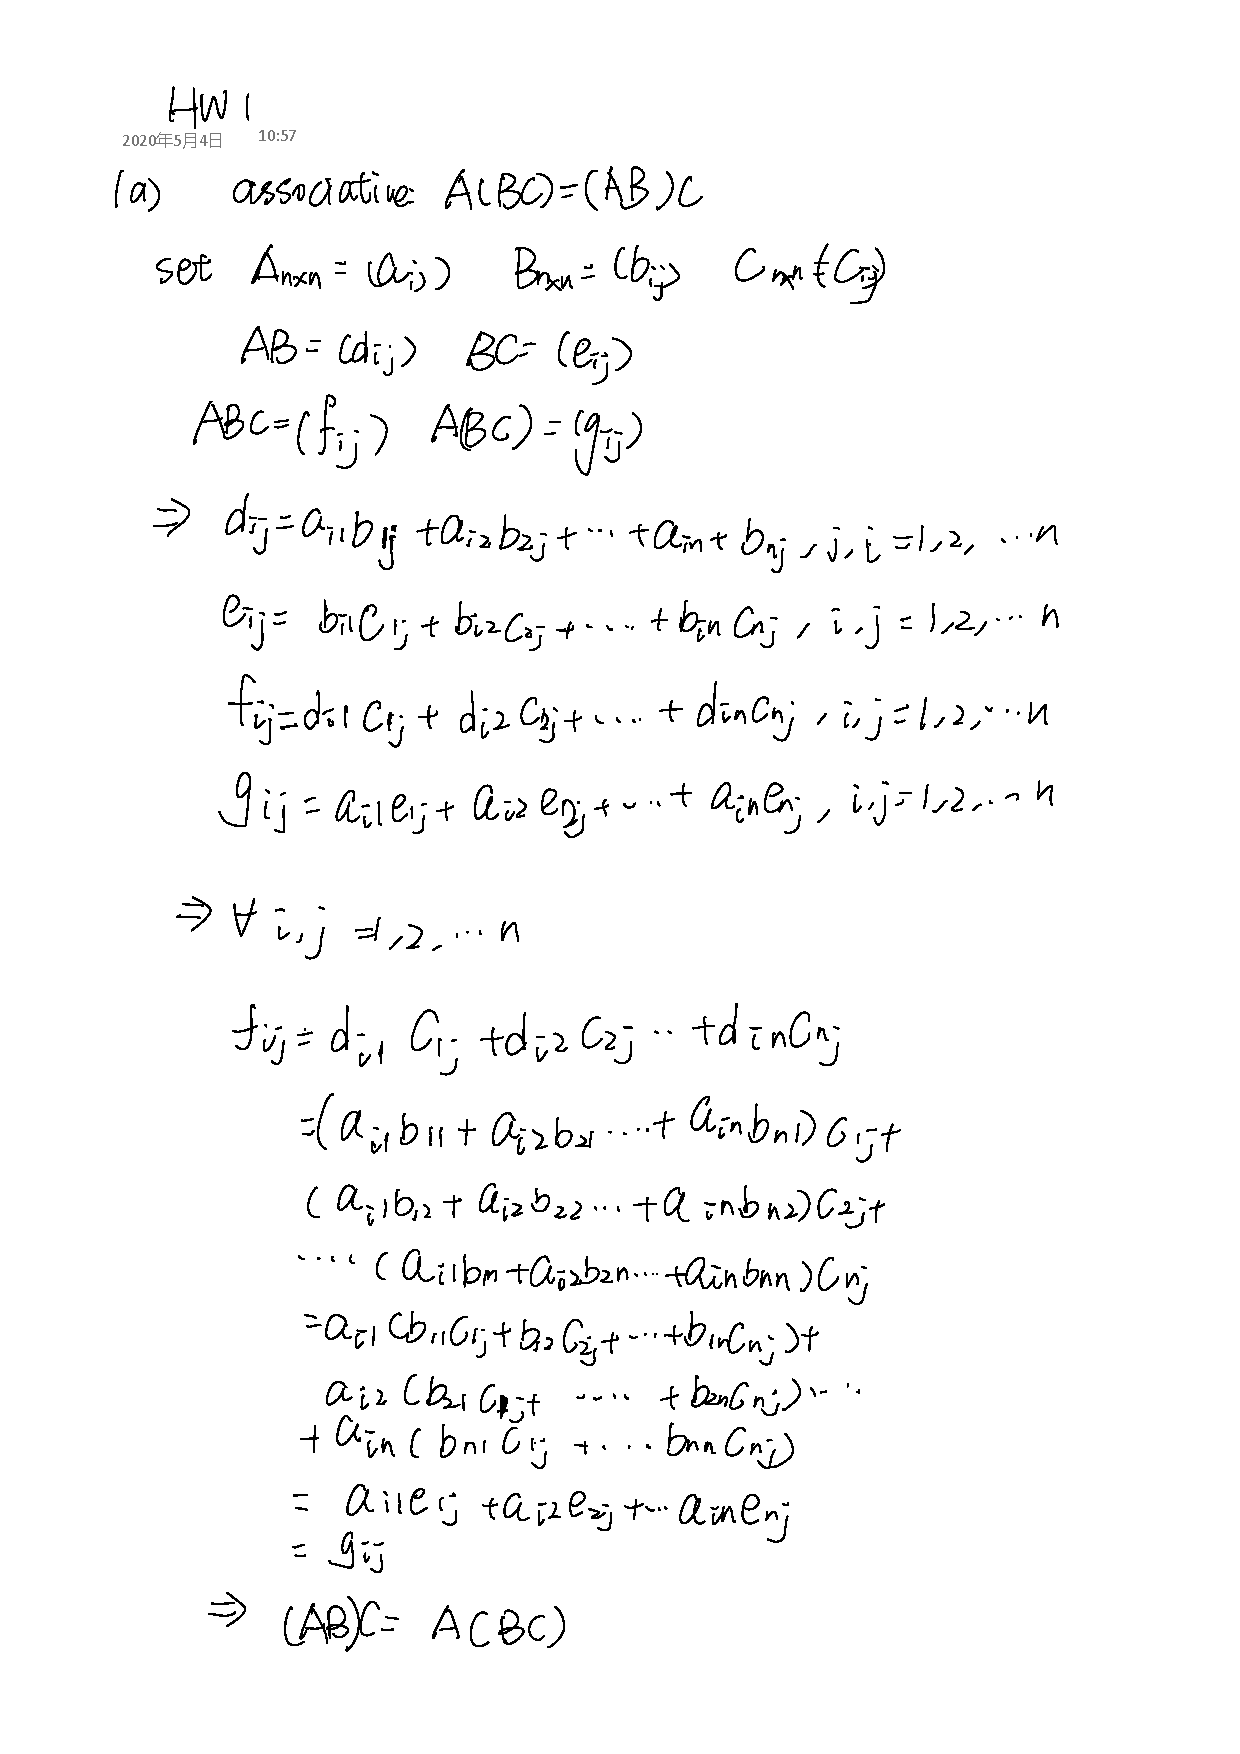
\includepdf[pages={1,2,3}]{sml1.pdf}
\subsubsection{1d}
Eigenvectors represent various linear transformations of the matrix,their corre-
sponding eigenvalues represent the degree of the linear transformation.A square
matrix in a high-dimensional space represents a set of linear transformations in
a high-dimensional space.These transformation include many transformations
of different degree and in different directions. Therefore, in order to simplify
the problem and retain as much transformation information as possible, we can
decompose the high dimensional matrix by use of eigenvalue and eigenvectors,
so as to approximately describe the square matrix. In machine learning ,com-
plex square matrix can be described with help of eigenvalues and eigenvectors.
SVD,PCA and Linear Discriminant Analysis involve eigenvalues and eigenvec-
tors.
\section{Task2}
\subsection{2a}
\subsubsection{1}
Exception
$$E_{\omega\sim p(\omega)}[f]=\sum_{w\in\Omega}{P(\omega)f(\omega)}$$
Variance
$$var=E[f^2]-E[f]^2$$
they are unlinear operator
\subsubsection{2}
$$E(A)=1\times\frac{4}{18}+2\times\frac{1}{18}+3\times\frac{6}{18}+4\times\frac{2}{18}+5\times\frac{1}{18}+6\times\frac{4}{18}=3.39$$
$$var(A)=\frac{(1-3.39)^2\times4+(2-3.39)^2\times1+(3-3.39)^2\times6+(4-3.39)^2\times2+(5-3.39)^2\times1+(6-3.39)^2\times4}{17}$$
$$=3.31$$
$$E(B)=2.78$$
$$var(B)=3.01$$ 
$$E(C)=3.44$$
$$var(C)=3.08$$
\subsubsection{3}
$$A:KL(p||q)=\sum P(x)log\frac{P(x)}{Q(x)}=0.19$$
$$B:KL(p||q)=0.25$$
$$C:KL(p||q)=0.02$$
C is closest to a fair, uniform die.
\subsection{2b}
suffer from cold is event x, suffer from back-pain is event y
$$p(y|x)=0.3$$
$$p(x)=0.03$$
$$p(y|!x)=0.1$$
$$p(y)=p(x,y)+p(!x,y)=p(y|x)\times p(x)+p(y|!x)\times p(!x)=0.106$$
$$p(x|y)=\frac{p(x,y)}{p(y)}=0.085$$
\subsection{2c}
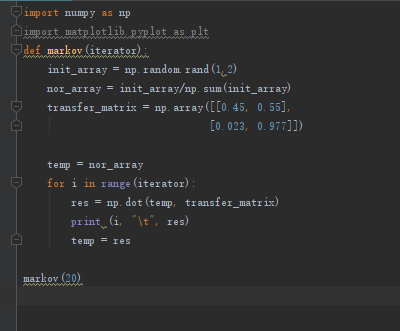
\includegraphics[scale=0.6]{1590578111(1).png}
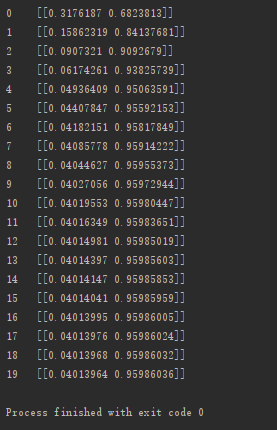
\includegraphics[scale=0.6]{1590578087(1).png}
The third generation has not changed significantly,the 21st has not changed.

My plan is failed.
\section{Task3}
\subsection{3a}
$$H(p)=\sum P(x)log\frac{1}{P(x)}=1.28$$
$$max H(p)=\sum0.25log\frac{1}{0.25}=2$$
The maximal entropy follows uniform distribution.
\subsection{3b}
\subsubsection{1}
$$min \ \sum_{i=1}^4p_i\log(p_i)$$
$$s.t.  6=\sum_{i=1}^42p_i i,(p_i-1)\leq0$$
\subsubsection{2}
$$max_{\alpha,\beta} L(p_i,\lambda,\beta)=\sum_{i=1}^4p_i\log(p_i)+\alpha\sum_{i=1}^4 (p_i-1)+\beta(\sum_{i=1}^42p_ii-6)$$
\subsubsection{3}
$$\frac{\partial L}{\partial p_i}=\log(p_i)+\frac{1}{ln2}+\alpha+2\beta i,\  i=1,2,3,4$$
$$\frac{\partial L}{\partial \alpha}=\sum_{i=1}^4 (p_i-1)$$
$$\frac{\partial L}{\partial \beta}=(\sum_{i=1}^42p_ii-6)$$
we need to solve the minimal value, but the $p_i-1$is not 0, we can adjust $\alpha_i$ to make L become $-\infty$.
\subsubsection{4}
$$\theta_{D}=min_{p_i}L$$
$$\frac{\partial L}{\partial p_i}=0,\  i=1,2,3,4$$
$$\alpha\sum_{i=1}^4 (p_i-1)=0$$
$$6=\sum_{i=1}^42p_i i$$
we can compute $\alpha=0$
\subsubsection{5}
steepest descent
\subsection{3c}
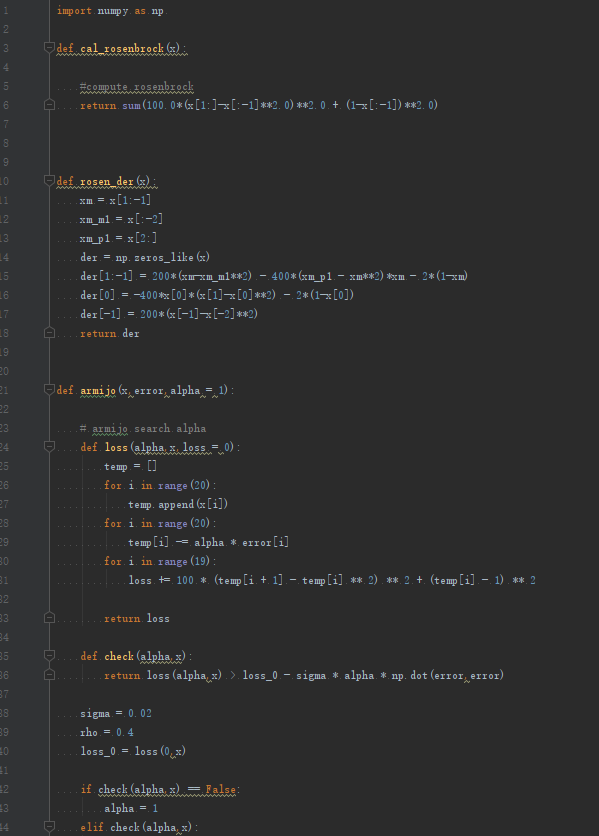
\includegraphics[scale=0.6]{1590807226(1).png}
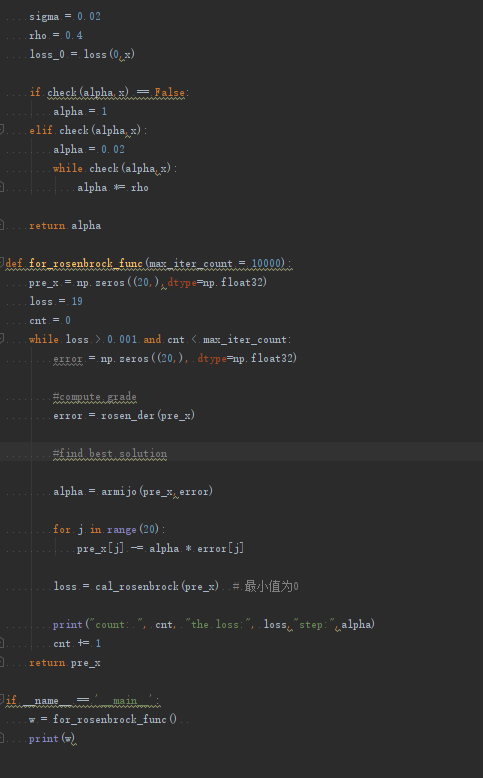
\includegraphics[scale=0.6]{1590807235(1).png}
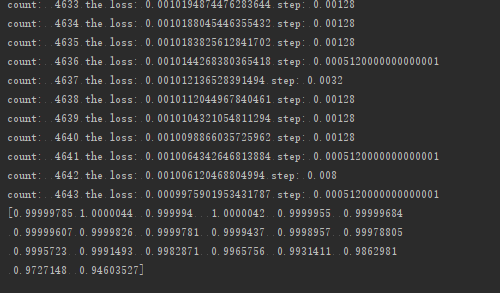
\includegraphics[scale=0.6]{1590807273(1).png}

in step 4642 we achieve x=[0.99999785 1.0000044  0.999994   1.0000042  0.9999955  0.99999684
0.99999607 0.9999826  0.9999781  0.9999437  0.9998957  0.99978805
0.9995723  0.9991493  0.9982871  0.9965756  0.9931411  0.9862981
0.9727148  0.94603527]
if the delta is too long, the plot will concussion. 
\subsection{3d}
\subsubsection{1}
Batch:
$$\theta_{j+1}=\theta-\alpha\delta_\theta J(\theta)$$
all the datas are used in the computing, so the result is exact but the calculation time is large and occupy much resource.
stochastic:
$$\theta_{j+1}=\theta-\alpha\delta_\theta J(\theta,x^i,y^i)$$
every iteration only uses oone point in SGD, so the need of calculation time is less . But not all iterations can reach to the global optimum.
Mini-Batch:
$$\theta_{j+1}=\theta-\alpha\delta_\theta J(\theta,x^{i:i+n},j^{i:i+n})$$
This allows a balance between calculated amount and computing time,but the convergence is not  very ideal.
\subsubsection{2}
When we use new data to iterate an inertia, we gives the old direction aweight too. The computing is stabler but not always useful when we need to run faster.
\end{document}